\subsubsection{Caso d'uso UC8.1.3.2: Creazione domanda a risposta multipla}
	\label{UC8.1.3.2}
	\begin{figure}[h]
		\centering
			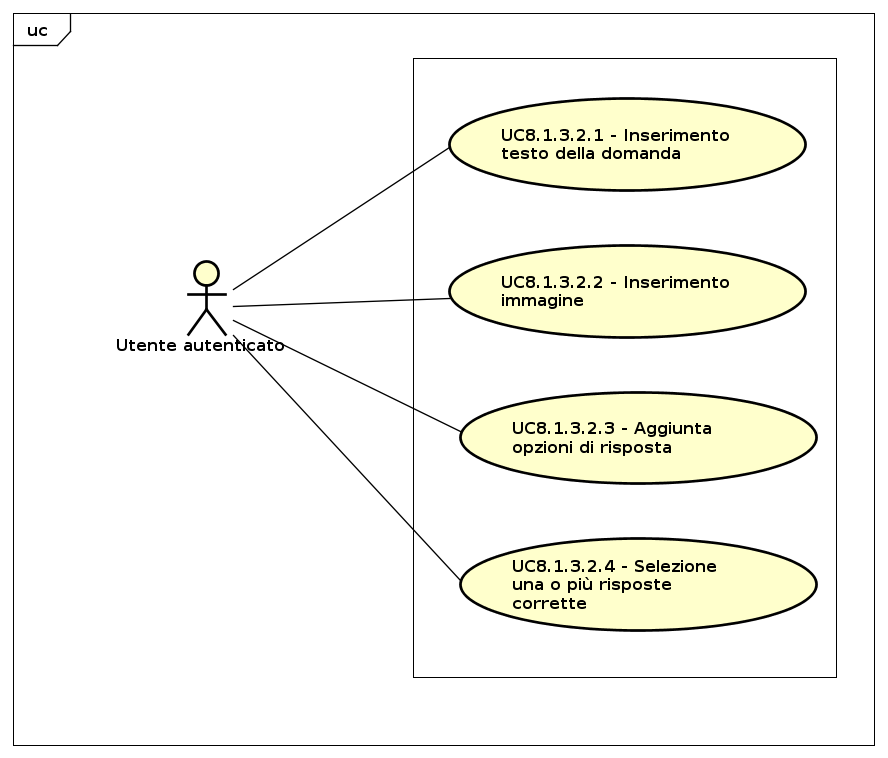
\includegraphics[scale=0.45,keepaspectratio]{UML/UC8_1_3_2.png}
		\caption{UC8.1.3.2: Creazione domanda a risposta multipla}
	\end{figure}
	\FloatBarrier
	\begin{itemize}
		\item
			\textbf{Attori}: utente autenticato, utente autenticato pro;
		\item		
			\textbf{Descrizione}: l'attore può creare domande a risposta multipla;
		\item
			\textbf{Precondizione}: l'attore ha selezionato la seguente funzionalità; 
		\item
			\textbf{Postcondizione}: l'attore ha creato una domanda a risposta multipla;
		\item
			\textbf{Scenario principale}:
	       		\begin{enumerate}
	       			\item
	       			l'attore può compilare il campo dati destinato alla scrittura del testo della domanda (UC8.1.3.2.1)
	       			\item
	       			l'attore può inserire un'immagine relativa al testo della domanda (UC8.1.3.2.2)
	       			\item
	       			l'attore può aggiungere almeno due opzioni di risposta (UC8.1.3.2.3);
					\item
					l'attore può indicare una o più risposte corrette (UC8.1.3.2.4).
	 			\end{enumerate}
	\end{itemize}

\subsubsection{Caso d'uso UC8.1.3.2.1: Inserimento testo della domanda}
	\begin{itemize}
		\item
			\textbf{Attori}: utente autenticato, utente autenticato pro;
		\item		
			\textbf{Descrizione}: l'attore può inserire il testo della domanda;
		\item
			\textbf{Precondizione}: l'attore ha selezionato la funzionalità di creazione di una domanda a risposta multipla; 
		\item
			\textbf{Postcondizione}: l'attore ha inserito il testo della domanda;
		\item
			\textbf{Scenario principale}: l'attore inserisce il testo della domanda. 
	 			
	\end{itemize}
	
\subsubsection{Caso d'uso UC8.1.3.2.2: Inserimento immagine}
	\begin{itemize}
		\item
			\textbf{Attori}: utente autenticato, utente autenticato pro;
		\item		
			\textbf{Descrizione}: l'attore può inserire un'immagine relativa al testo della domanda;
		\item
			\textbf{Precondizione}: l'attore ha selezionato la funzionalità di creazione di una domanda a risposta multipla; 
		\item
			\textbf{Postcondizione}: l'attore ha inserito l'immagine;
		\item
			\textbf{Scenario principale}: l'attore inserisce l'immagine. 	
	\end{itemize}
	
	
\subsubsection{Caso d'uso UC8.1.3.2.3: Aggiunta opzioni di risposta}
	\label{UC8.1.3.2.3}
	\begin{figure}[h]
		\centering
			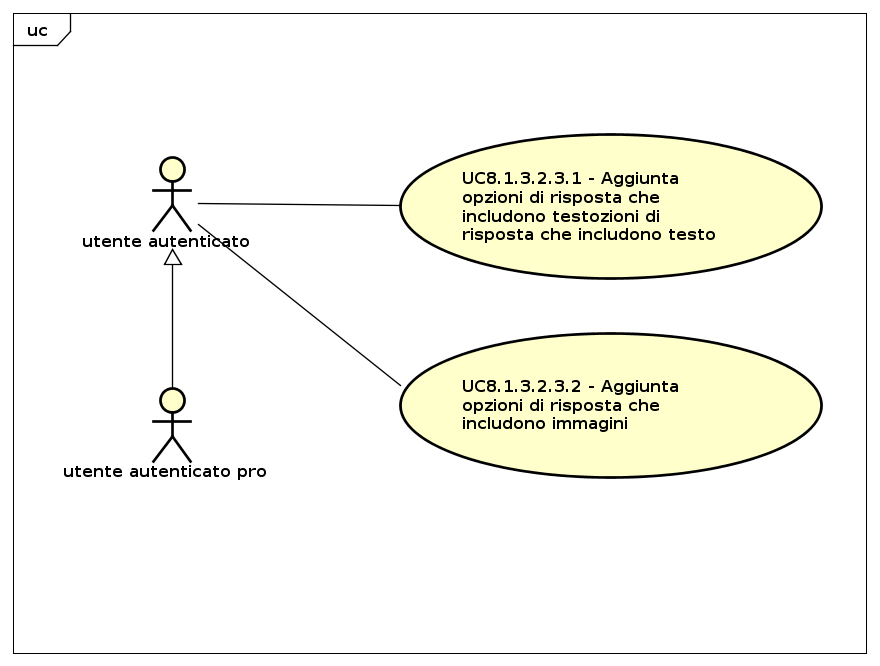
\includegraphics[scale=0.45,keepaspectratio]{UML/UC8_1_3_2_3.png}
		\caption{UC8.1.3.2.3: Aggiunta opzioni di risposta}
	\end{figure}
	\FloatBarrier
	\begin{itemize}
		\item
			\textbf{Attori}: utente autenticato, utente autenticato pro;
		\item		
			\textbf{Descrizione}: l'attore può aggiungere almeno due opzioni di risposta;
		\item
			\textbf{Precondizione}: l'attore ha selezionato la funzionalità di creazione di una domanda a risposta multipla; 
		\item
			\textbf{Postcondizione}: l'attore ha aggiunto due o più opzioni di risposta;
		\item
			\textbf{Scenario principale}:
	       		\begin{enumerate}
	       			\item
	       			L'attore può aggiungere opzioni di risposta che includono testo (UC8.1.3.2.3.1);
					\item
					L'attore può aggiungere opzioni di risposta che includono immagini (UC8.1.3.2.3.2).
	 			\end{enumerate}
	\end{itemize}	
	
\subsubsection{Caso d'uso UC8.1.3.2.3.1: Aggiunta opzioni di risposta che includono testo}
	\begin{itemize}
		\item
			\textbf{Attori}: utente autenticato, utente autenticato pro;
		\item		
			\textbf{Descrizione}: l'attore può aggiungere almeno due opzioni di risposta che includono testo;
		\item
			\textbf{Precondizione}: l'attore ha selezionato la funzionalità di creazione di domande a risposta multipla con opzioni di risposta che includono testo; 
		\item
			\textbf{Postcondizione}: l'attore ha aggiunto due o più opzioni di risposta che includono testo;
		\item
			\textbf{Scenario principale}: l'attore aggiunge due o più opzioni di risposta che includono testo. 			
	\end{itemize}	
	
\subsubsection{Caso d'uso UC8.1.3.2.3.2: Aggiunta opzioni di risposta che includono immagini}
	\begin{itemize}
		\item
			\textbf{Attori}: utente autenticato, utente autenticato pro;
		\item		
			\textbf{Descrizione}: l'attore può aggiungere almeno due opzioni di risposta che includono immagini;
		\item
			\textbf{Precondizione}: l'attore ha selezionato la funzionalità di creazione di domande a risposte multipla con opzioni di risposta che includono immagini; 
		\item
			\textbf{Postcondizione}: l'attore hanno aggiunto due o più opzioni di risposta che includono immagini;
		\item
			\textbf{Scenario principale}: l'attore aggiunge due o più opzioni di risposta che includono immagini. 			
	\end{itemize}
	
\subsubsection{Caso d'uso UC8.1.3.2.4: Selezione una o più risposte corrette}
	\begin{itemize}
		\item
			\textbf{Attori}: utente autenticato, utente autenticato pro;
		\item		
			\textbf{Descrizione}:l'attore può selezionare una o più risposte corrette;
		\item
			\textbf{Precondizione}: l'attore ha selezionato la funzionalità di creazione di domande a risposta multipla; 
		\item
			\textbf{Postcondizione}: l'attore ha selezionato una o più risposte corrette;
		\item
			\textbf{Scenario principale}: l'attore selezionano una o più risposte corrette. 			
	\end{itemize}

	
	
	
	
	
	
	